\documentclass[12pt]{article}
\usepackage{amsmath}
\usepackage{amssymb}
\usepackage{geometry}
\usepackage{amsmath, amsfonts, bm, graphicx}
\usepackage{tabularx}
\usepackage{booktabs} 
\usepackage{float}
\usepackage{enumitem}
\geometry{margin=1in}

\title{}
\date{}
\author{}

\begin{document}
\subsection*{\boxed{\text{HW 3 - Zeshui Song}}}

\section*{4.6}
\vspace{-2em}
\begin{center}
    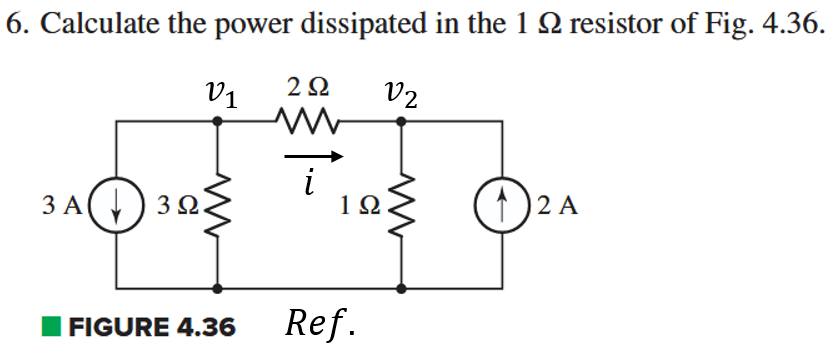
\includegraphics[width=0.8\textwidth]{4-6.png}
\end{center}
\vspace{-1em}
Using nodal analysis at node 1:
\[[-3\,\text{A}]=\frac{v_1}{[3\,\Omega]} + \frac{v_1-v_2}{[2\,\Omega]} \quad \implies \quad -3 = \frac{5}{6} v_1 - \frac{1}{2} v_2\]
At node 2:
\[\frac{v_1-v_2}{[2\,\Omega]} = \frac{v_2}{[1\,\Omega]} - [2\,\text{A}] \quad \implies \quad -2 = \frac{1}{2} v_1 - \frac{3}{2} v_2\]
Solving the system of equations, we get $v_1 = -7/2\,\text{V}$ and $v_2 = 1/6\,\text{V}$.\\\\
The power dissipated by the $1\,\Omega$ resistor is then
\[P = VI = \frac{v_2^2}{R} = \frac{[1/6\,\text{V}]^2}{[1\,\Omega]} = 0.02777\,\text{W} \]
\[\boxed{P=0.0278\,\text{W}}\]

\section*{4.12}
\vspace{-2em}
\begin{center}
    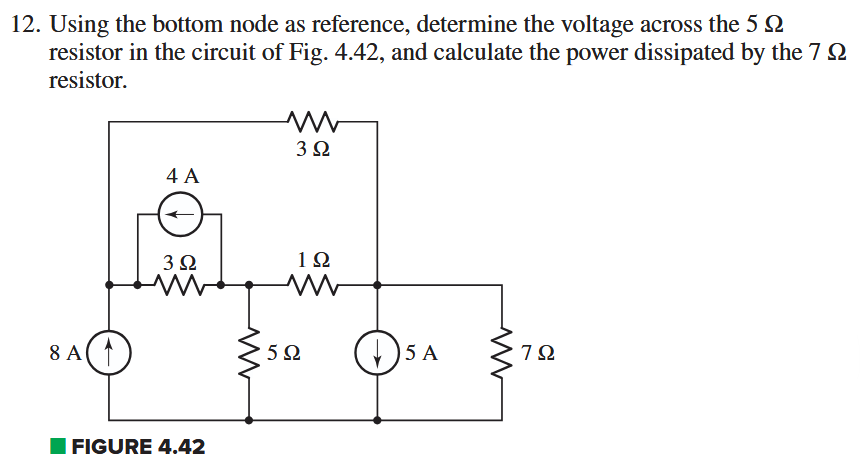
\includegraphics[width=0.8\textwidth]{4-12.png}
\end{center}
\vspace{-1em}
Redrawing the circuit slightly and labeling the nodes:
\begin{center}
    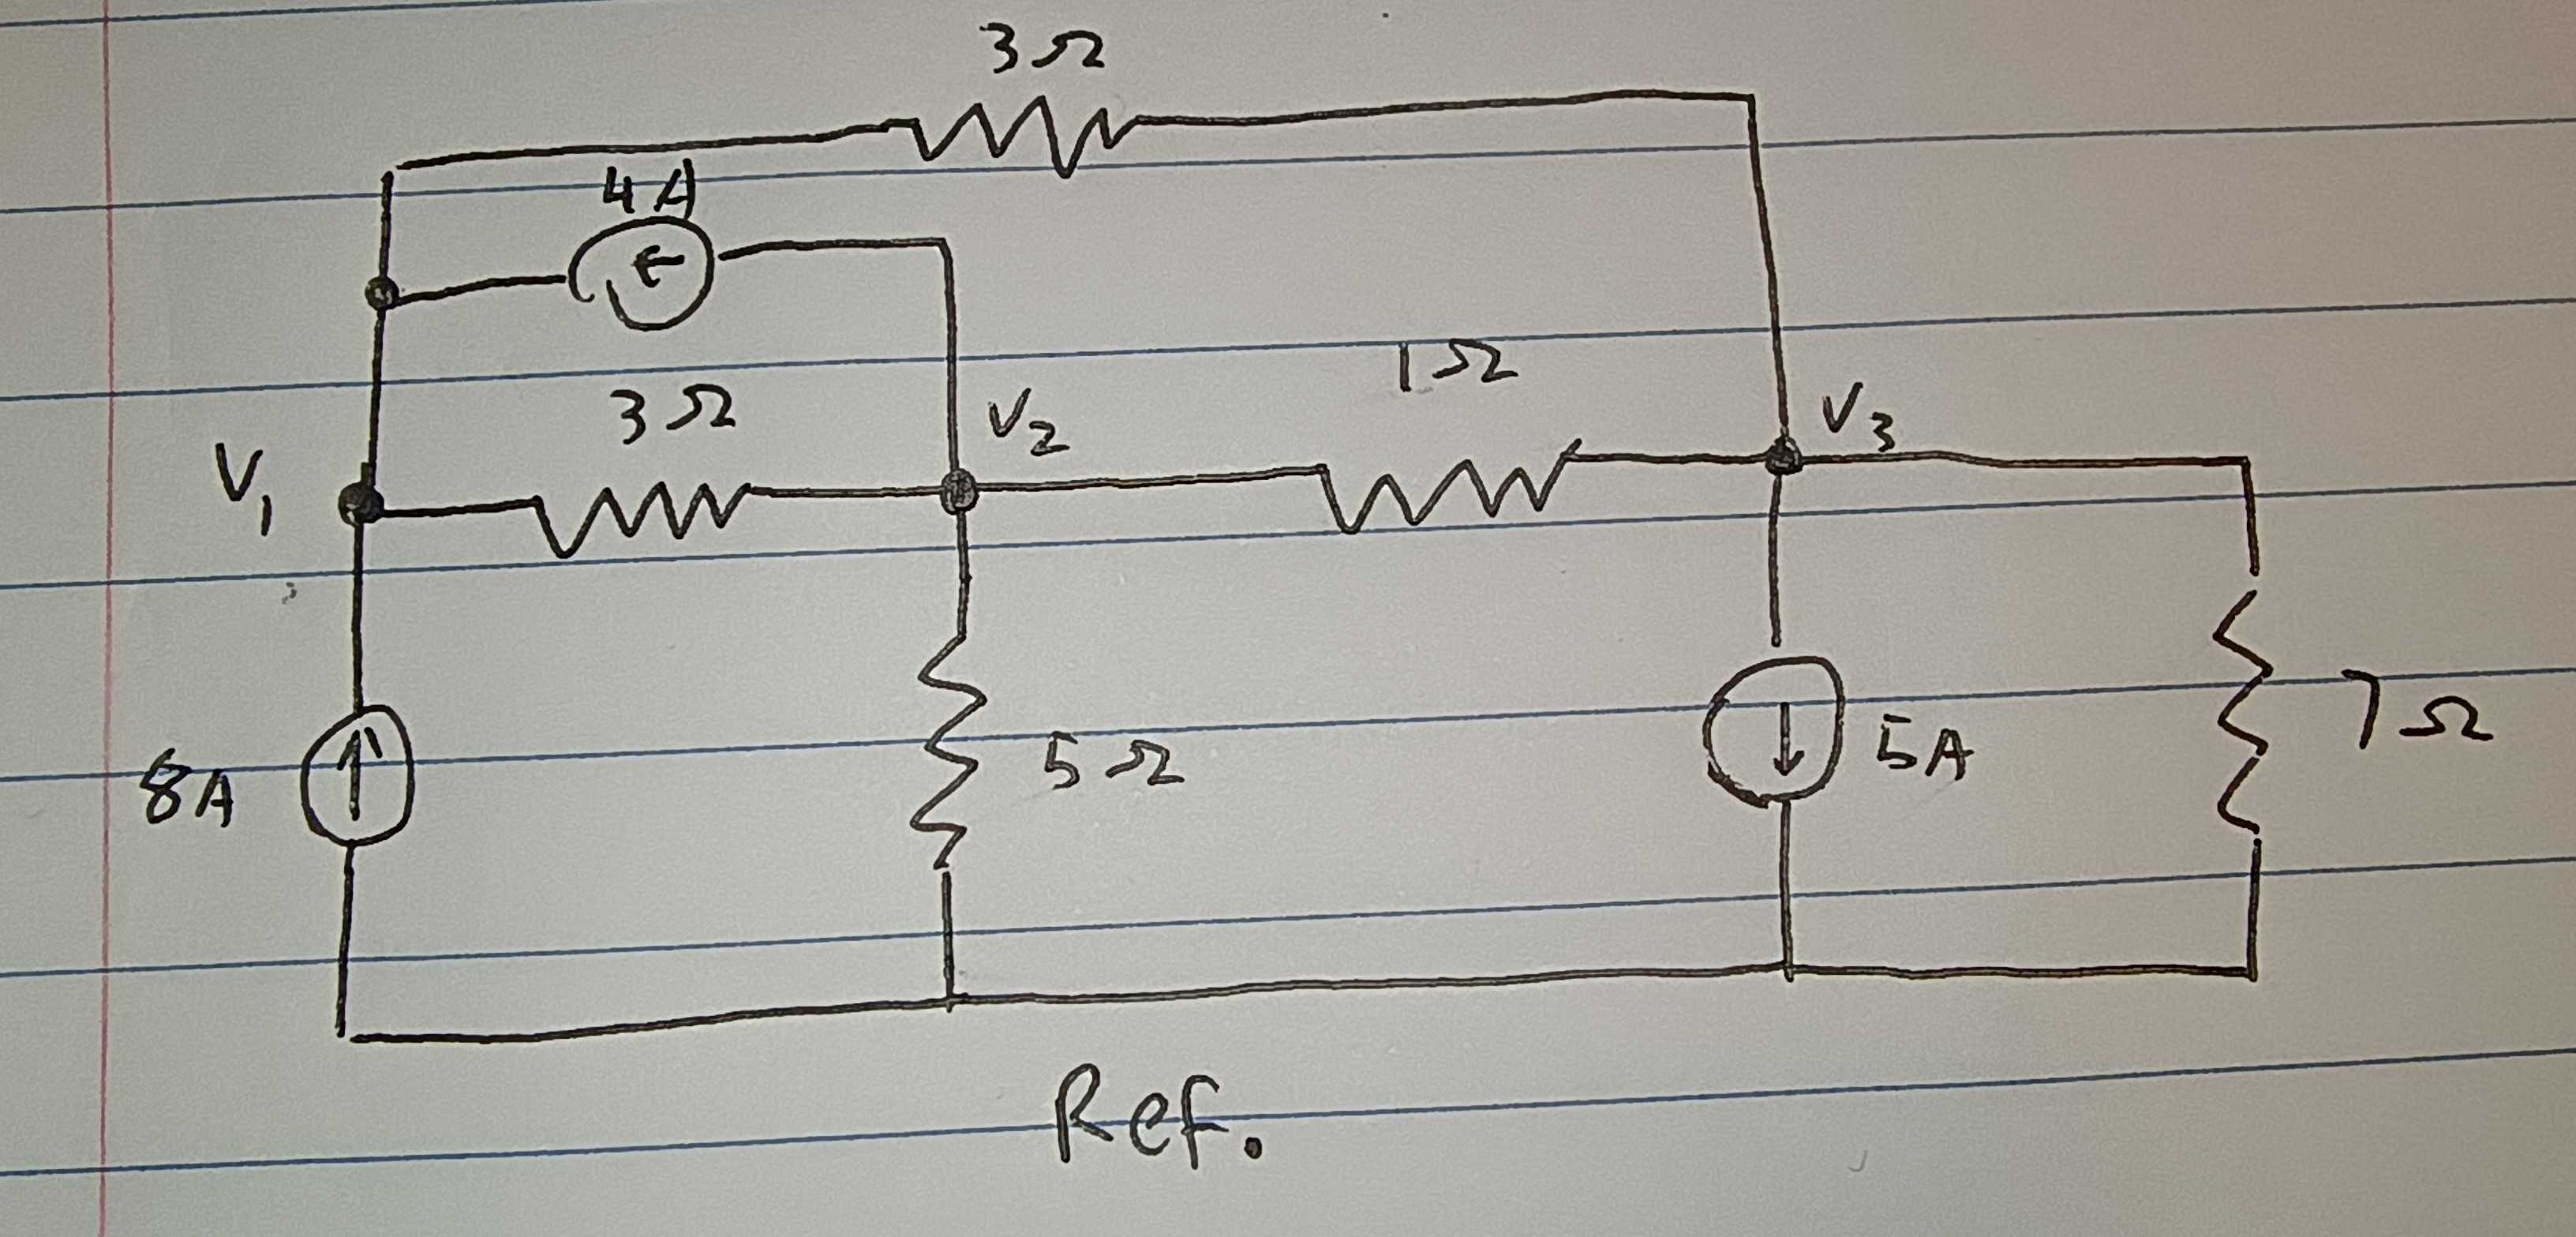
\includegraphics[width=0.6\textwidth]{4-12_1.jpg}
\end{center}
At node 1:
\[[8\,\text{A}] = \frac{v_1 - v_3}{[3\,\Omega]} - [4\,\text{A}]+\frac{v_1-v_2}{[3\,\Omega]}\quad\implies\quad
12 = \frac{2}{3}v_1 -\frac{1}{3}v_2 - \frac{1}{3}v_3\]
At node 2:
\[\frac{v_1-v_2}{[3\,\Omega]}=[4\,\text{A}]+\frac{v_2-v_3}{[1\,\Omega]}+\frac{v_2}{[5\,\Omega]}\quad\implies\quad
4 = \frac{1}{3}v_1 - \frac{23}{15}v_2 + v_3\]
At node 3:
\[\frac{v_2-v_3}{[1\,\Omega]} + \frac{v_1-v_3}{[3\,\Omega]}= [5\,\text{A}] + \frac{v_3}{[7\,\Omega]}\quad\implies\quad
5 = \frac{1}{3}v_1 + v_2 - \frac{31}{21}v_3\]
Solving the system of equations, we get $v_1 = 26.733\,\text{V}$, $v_2 = 8.833\,\text{V}$, and $v_3 = 8.633\,\text{V}$.\\\\
The power dissipated by the $7\,\Omega$ resistor is then
\[P = VI = \frac{v_3^2}{R} = \frac{[8.633\,\text{V}]^2}{[7\,\Omega]} = 10.54\,\text{W}\]
\[\boxed{P=10.64\,\text{W}}\]
and the voltage across the $5\,\Omega$ resistor is
\[\boxed{v_3 = 8.633\,\text{V}}\]

\section*{4.20}
\vspace{-2em}
\begin{center}
    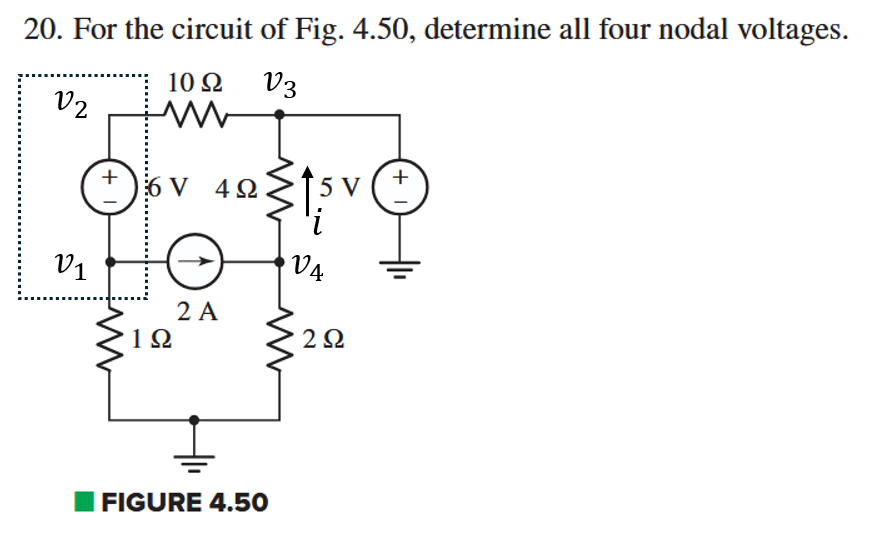
\includegraphics[width=0.8\textwidth]{4-20.png}
\end{center}
\vspace{-1em}
Using a super node around the voltage source at nodes 1 and 2:
\[v_2-v_1 = [6\,\text{V}] \quad\implies\quad
6 = -1v_1 + v_2\]
\[\frac{0-v_1}{[1\,\Omega]} = \frac{v_2-v_3}{[10\,\Omega]} + [2\,\text{A}]\quad\implies\quad 
2 = -v_1 - \frac{1}{10}v_2 + \frac{1}{10}v_3\]
At node 3:
\[v_3 = [5\,\text{V}]\]
At node 4:
\[[2\,\text{A}] = \frac{v_4}{[2\,\Omega]} + \frac{v_4-v_3}{[4\,\Omega]}\quad\implies\quad
2 = -\frac{1}{4}v_3+\frac{3}{4}v_4\]
Solving the system of equations, we get 
\[\boxed{v_1 = -1.909\,\text{V}$, $v_2 = 4.0909\,\text{V}$, $v_3 = 5\,\text{V}$, and $v_4 = 4.333\,\text{V}}\]

\section*{4.32}
\vspace{-2em}
\begin{center}
    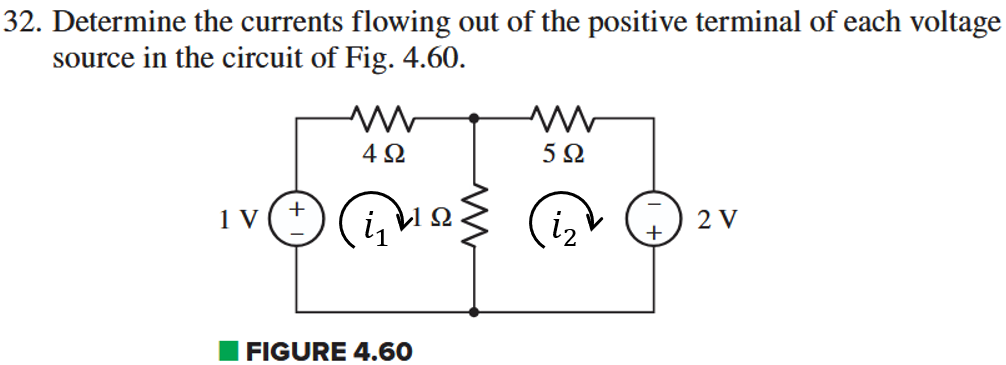
\includegraphics[width=0.8\textwidth]{4-32.png}
\end{center}
\vspace{-1em}
Using mesh analysis on the left loop:
\[[1\,\text{V}] - [4\,\Omega]i_1 - [1\,\Omega](i_1-i_2) = 0 \quad \implies \quad 1 = 5i_1 - i_2\]
Using mesh analysis on the right loop:
\[-[1\,\Omega](i_2-i_1)-[5\,\Omega]i_2+[2\,\text{V}] = 0  \quad \implies \quad 2 = -i_1 + 6i_2\]
Solving the system of equations, we get $i_1 = 0.2758\,\text{A}$ and $i_2 = 0.3793\,\text{A}$.

\section*{4.36}
\vspace{-2em}
\begin{center} 
    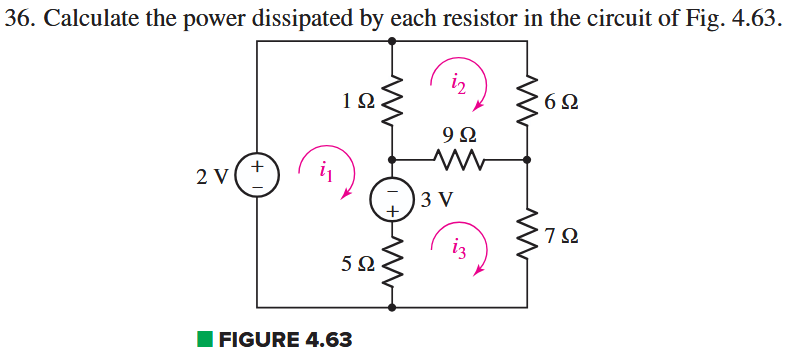
\includegraphics[width=0.8\textwidth]{4-36.png}
\end{center}
\vspace{-1em}
Mesh 1:
\[[2\,\text{V}]-[1\,\Omega](i_1 - i_2) + [3\,\text{V}] - [5\,\Omega](i_1-i_3) = 0 \quad \implies \quad 
5 = 6i_1 -i_2 -5i_3\]
Mesh 2:
\[[1\,\Omega](i_2-i_1) - [6\,\Omega]i_2 - [9\,\Omega](i_2-i_3)\quad\implies\quad
0=i_1+14i_2-9i_3\]
Mesh 3:
\[-[5\,\Omega](i_3-i_1) - [3\,\text{V}] - [9\,\Omega](i_3-i_2)-[7\,\Omega]i_3 = 0 \quad\implies\quad
-3 = -5i_1 -9i_2 +21i_3\]
Solving the system of equations, we get $i_1 = 0.8724\,\text{A}$, $i_2 = -0.0284\,\text{A}$, and $i_3 = 0.0526\,\text{A}$.\\\\
Power dissipated by the $1\Omega$ resistor:
\[\boxed{P_{1\Omega} = Vi=(i_1-i_2)^2R = [0.8724-(-0.0284)\,\text{A}]^2 \cdot [1\,\Omega] = 0.8114\,\text{W}}\]

Power dissipated by the $5\Omega$ resistor:
\[\boxed{P_{5\Omega} = Vi=(i_1-i_3)^2R = [0.8724-0.0526\,\text{A}]^2 \cdot [5\,\Omega] = 3.360\,\text{W}}\]

Power dissipated by the $9\Omega$ resistor:
\[\boxed{P_{9\Omega} = Vi=(i_3-i_2)^2R = [0.0526-(-0.0284)\,\text{A}]^2 \cdot [9\,\Omega] = 0.0590\,\text{W}}\]

Power dissipated by the $6\Omega$ resistor:
\[\boxed{P_{6\Omega} = Vi=(i_2)^2R = [0.0284\,\text{A}]^2 \cdot [6\,\Omega] = 0.0048\,\text{W}}\]

Power dissipated by the $7\Omega$ resistor:
\[\boxed{P_{7\Omega} = Vi=(i_3)^2R = [0.0526\,\text{A}]^2 \cdot [7\,\Omega] = 0.0193\,\text{W}}\]

\section*{4.46}
\vspace{-2em}
\begin{center} 
    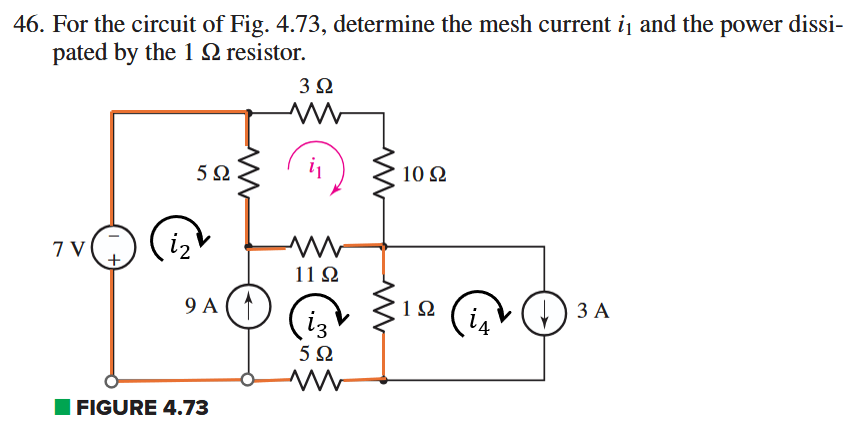
\includegraphics[width=0.8\textwidth]{4-46.png}
\end{center}
\vspace{-1em}
Orange supermesh:
\[i_3-i_2 = [9\,\text{A}] \quad\implies\quad
9 = -i_2 + i_3\]
\[-[7\,\text{V}] - [5\,\Omega](i_2-i_1) - [11\,\Omega](i_3-i_1) - [1\,\Omega](i_3 - i_4) - [5\,\Omega]i_3 =0 \quad\implies\quad
7 = 16i_1 -5i_2 -17i_3+i_4\]
Mesh 1:
\[-[5\,\Omega](i_1-i_2)-[3\,\Omega]i_1 - [10\,\Omega]i_1 - [11\,\Omega](i_1-i_3) = 0 \quad\implies\quad
-29i_2 +5i_2 +11i_3 = 0\]
Mesh 4:
\[i_4 = [3\,\text{A}] \quad\implies\quad 
3=i_4\]
Solving the system of equations, we get $i_1 = -0.8743\,\text{A}$, $i_2 = -7.7722\,\text{A}$, $i_3 = 1.2277\,\text{A}$, and $i_4 = 3\,\text{A}$.\\\\
Power dissipated by the $1\Omega$ resistor:
\[\boxed{P_{1\Omega} = Vi=(i_3-i_4)^2R = [1.2277-3\,\text{A}]^2 \cdot [1\,\Omega] = 3.141\,\text{W}}\]
\[\boxed{i_1 = -0.8743\,\text{A}}\]

\section*{4.56}
\vspace{-2em}
\begin{center}
    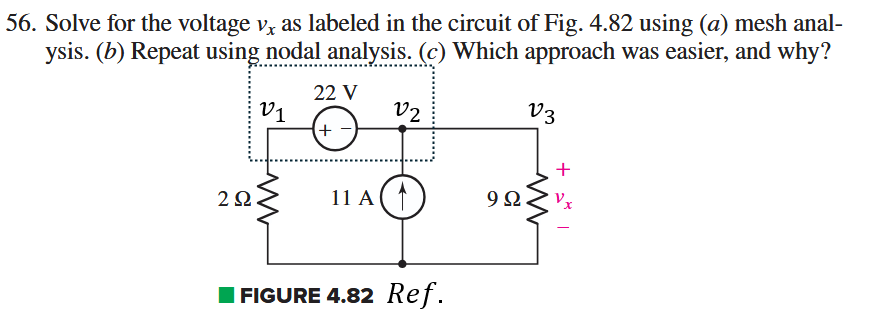
\includegraphics[width=0.8\textwidth]{4-56.png}
\end{center}
\vspace{-1em}
\textbf{(a)} Mesh analysis\\
Supermesh:
\[-[2\,\Omega]i_1 -[22\,\text{V}] - [9\,\Omega](i_2) = 0 \quad\implies\quad
22 = -2i_1 -9i_2\]
\[i_2-i_1 = [11\,\text{A}]\quad\implies\quad
11 = -i_1 + i_2\]
Solving the system of equations, we get $i_1 = -11\,\text{A}$ and $i_2 = 0\,\text{A}$.\\\\
Thus the voltage across the $9\,\Omega$ resistor is
\[\boxed{v_{9\Omega} = i_2 \cdot R = 0\,\text{A} \cdot [9\,\Omega] = 0\,\text{V}}\]
\textbf{(b)} Node analysis\\
At the 1-2 supernode:
\[v_1 - v_2=[22\,\text{V}]\quad\implies\quad 22 = v_1 - v_2\]
\[[11\,\text{A}] = \frac{v_1}{[2\,\Omega]} + \frac{v_2}{[9\,\Omega]}\quad\implies\quad
11 = \frac{1}{2}v_1 + \frac{1}{9}v_2\]
Node 3 is connected to the supernode, so there is no KCL equation for it.
Solving the system of equations, we get $v_1 = 22\,\text{V}$, $v_2 = 0\,\text{V}$, and $v_3 = v_2 = 0\,\text{V}$.\\\\
Thus the voltage across the $9\,\Omega$ resistor is
\[\boxed{v_{9\Omega} = v_3 = 0\,\text{V}}\]
\textbf{(c)} The mesh analysis was easier for me because it's the same amount of equations, but the supernode in the node analysis got me tripped up.

\section*{4.57}
\vspace{-2em}
\begin{center}  
    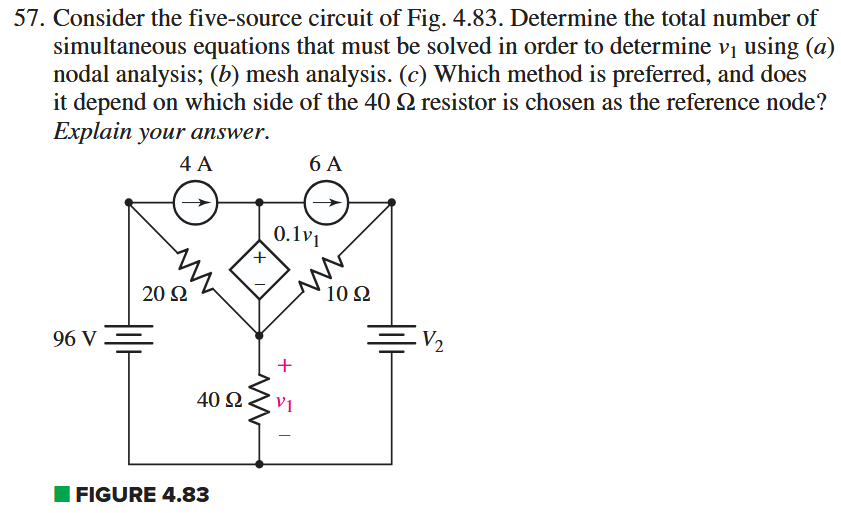
\includegraphics[width=0.8\textwidth]{4-57.png}
\end{center}
\vspace{-1em}
\textbf{(a)} For nodal analysis, we have a supernode around the 0.1$v_1$ voltage source and if we place reference node bottom wire, then we will have defined the leftmost and rightmost nodes. Thus we will only have 2 eqns to solve for with the supernode.\\\\
\textbf{(b)} For mesh analysis, we would have a supermesh after cutting out the 2 current sources. This would leave us with 2 equations to solve for the supermesh as the current in from the current sources are known.\\\\
\textbf{(c)} I think the nodal analysis is easier for this problem because the multiple current sources makes the mesh analysis more difficult. The reference node needs to be on the negative terminal of the 40 $\Omega$ resistor because it is needed to remove 2 unknown voltages.

\section*{5.3}
\vspace{-2em}
\begin{center}
    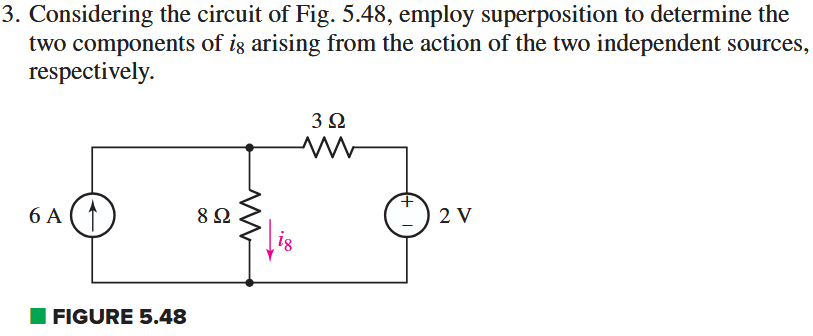
\includegraphics[width=0.8\textwidth]{5-3.png}
\end{center}
\vspace{-1em}
Turning off the voltage source (use node analysis):
\[[6\,\text{A}] = \frac{v_1}{[8\,\Omega]} + \frac{v_1}{[3\,\Omega]} \quad\implies\quad v_1 = [13.090\,\text{V}]\]
\[i_8' = \frac{v_1}{[8\,\Omega]} = \frac{13.090}{8} = [1.6363\,\text{A}]\]
Turning off the current source:
\[R_{\text{eq}} = [3\,\Omega] + [8\,\Omega] = [11\,\Omega]\]
\[i_8''=\frac{[2\,\text{V}]}{[11\,\Omega]} = [0.1818\,\text{A}]\]
Superposition:
\[\boxed{i_8 = i_8' + i_8'' = [1.6363 + 0.1818]\,\text{A} = [1.8181\,\text{A}]}\]

\section*{5.5}
\vspace{-2em}
\begin{center}
    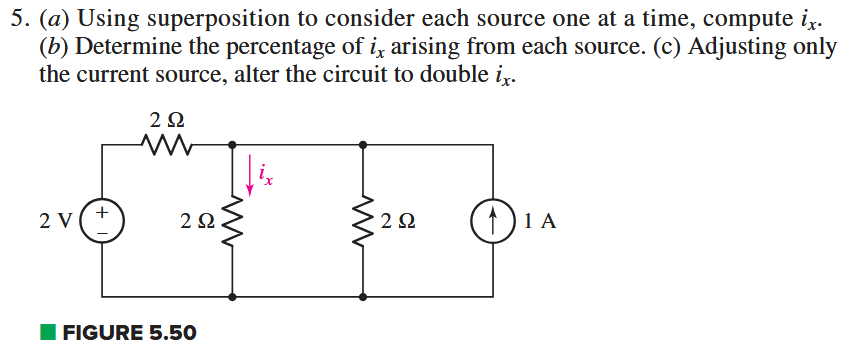
\includegraphics[width=0.8\textwidth]{5-5.png}
\end{center}
\vspace{-1em}
\textbf{(a)}\\
Turning off the voltage source:
\begin{center}
    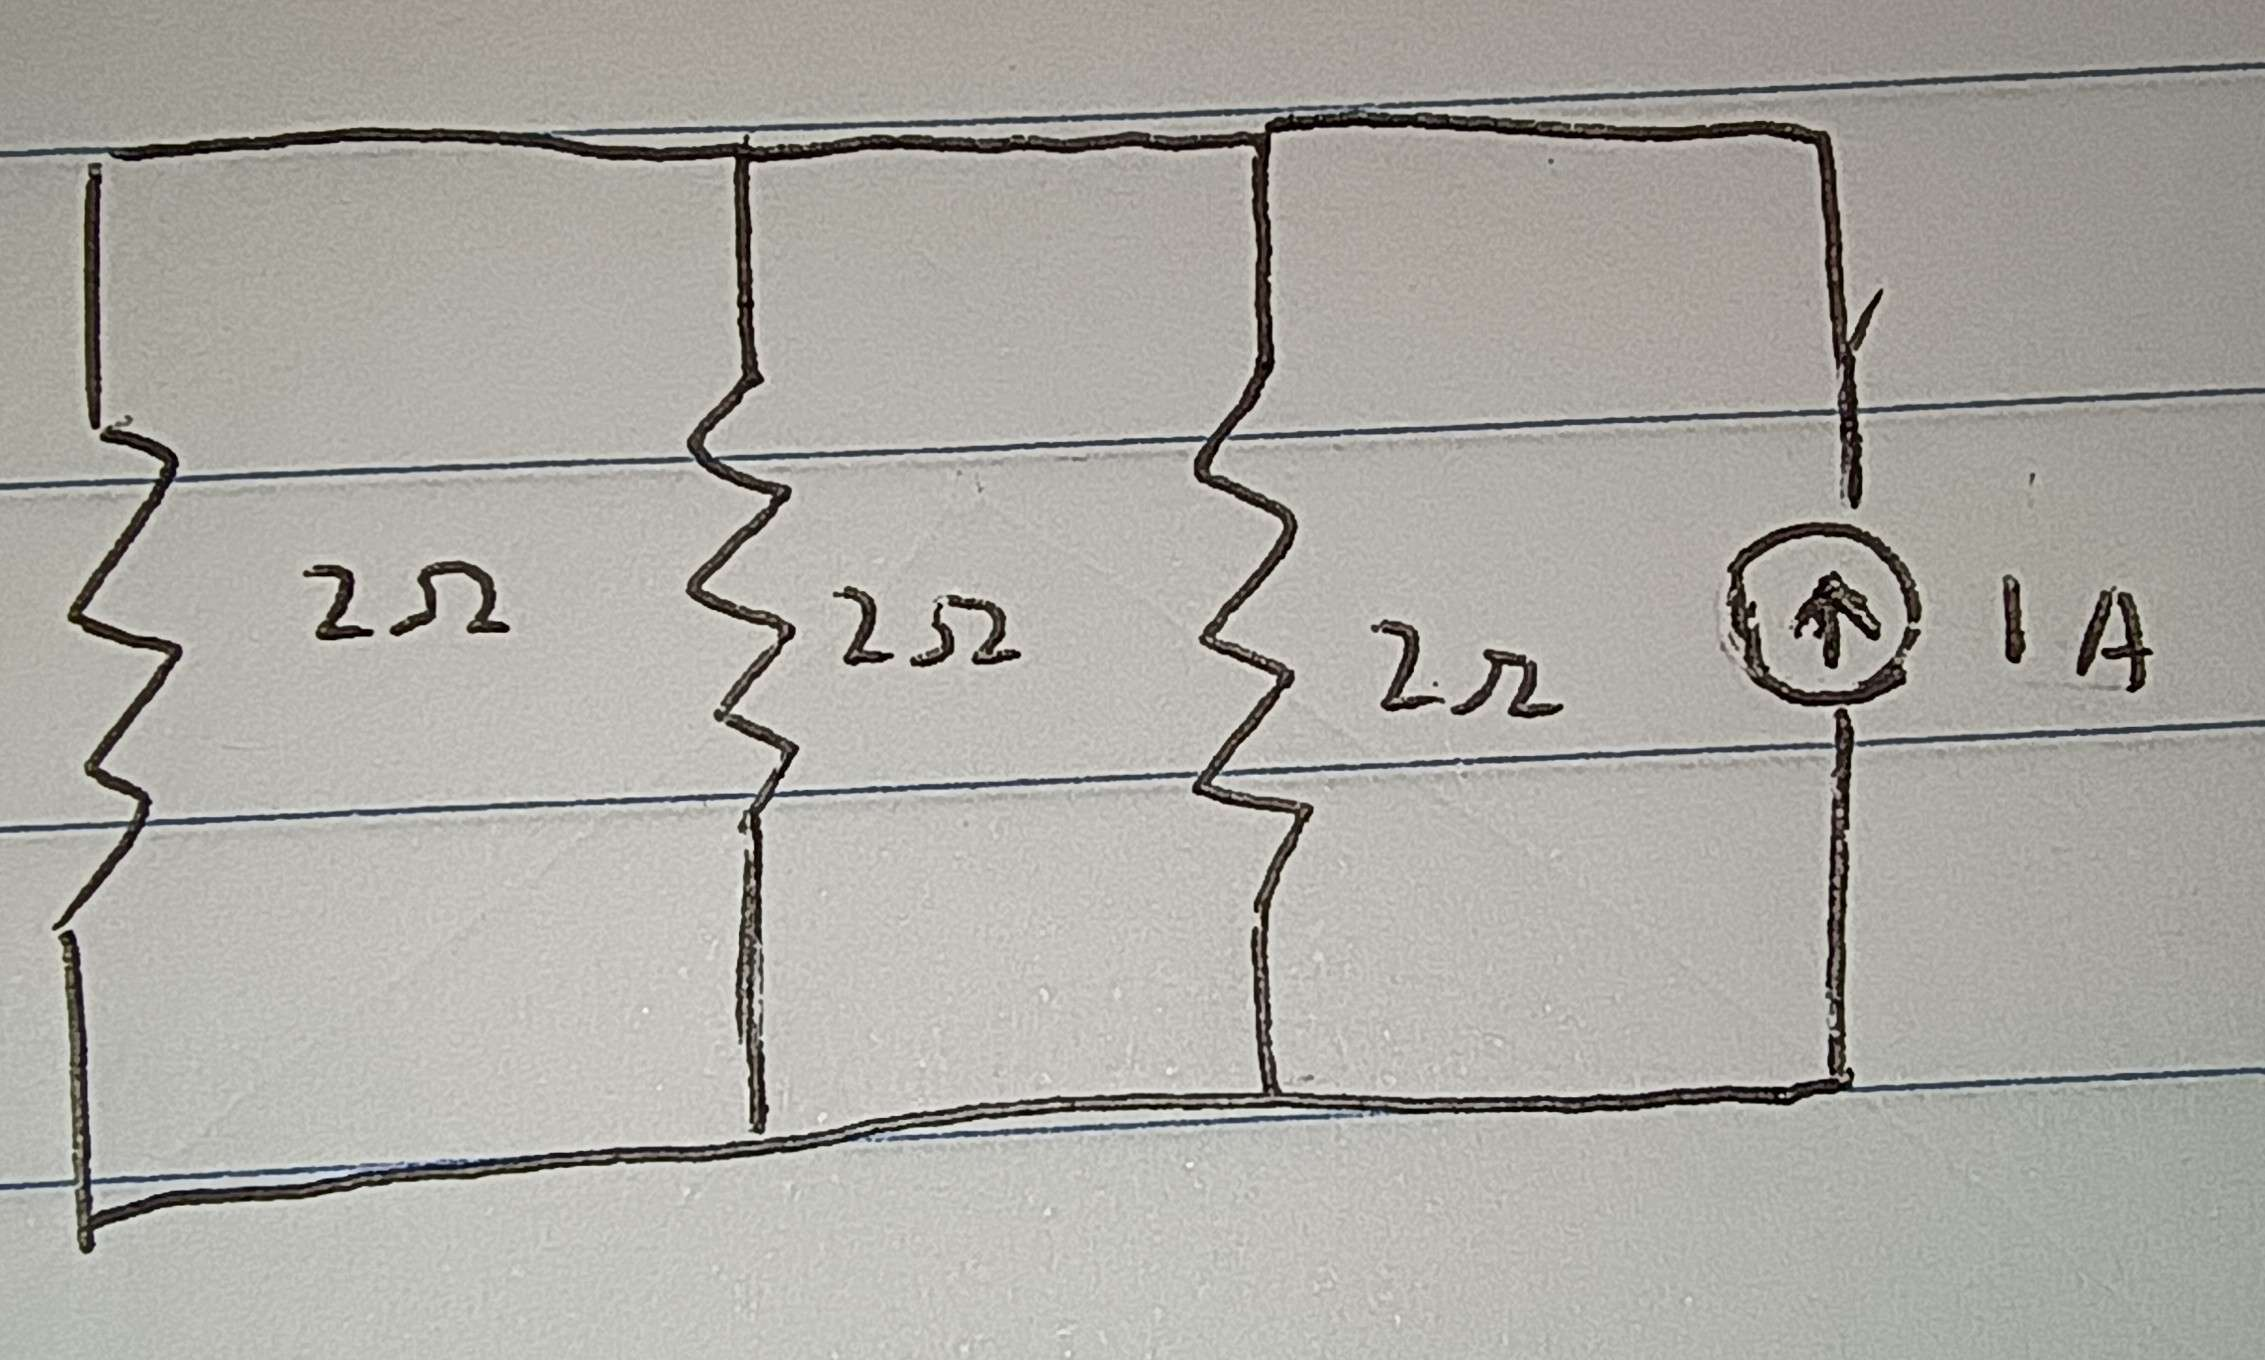
\includegraphics[width=0.6\textwidth]{5-5-1.jpg}
\end{center}
Combine the other two parallel resistors:
\[R_{\text{eq}} = \frac{[2+2\,\Omega]}{[2\cdot2\,\Omega]} = 1\,\Omega\]
Using the current division rule:
\[i_x' = \frac{[1\,\Omega]}{[1+2\,\Omega]} \cdot [1\,\text{A}] = \frac{1}{3} \cdot 1 = 0.3333\,\text{A}\]
Turning off the current source:
\begin{center}
    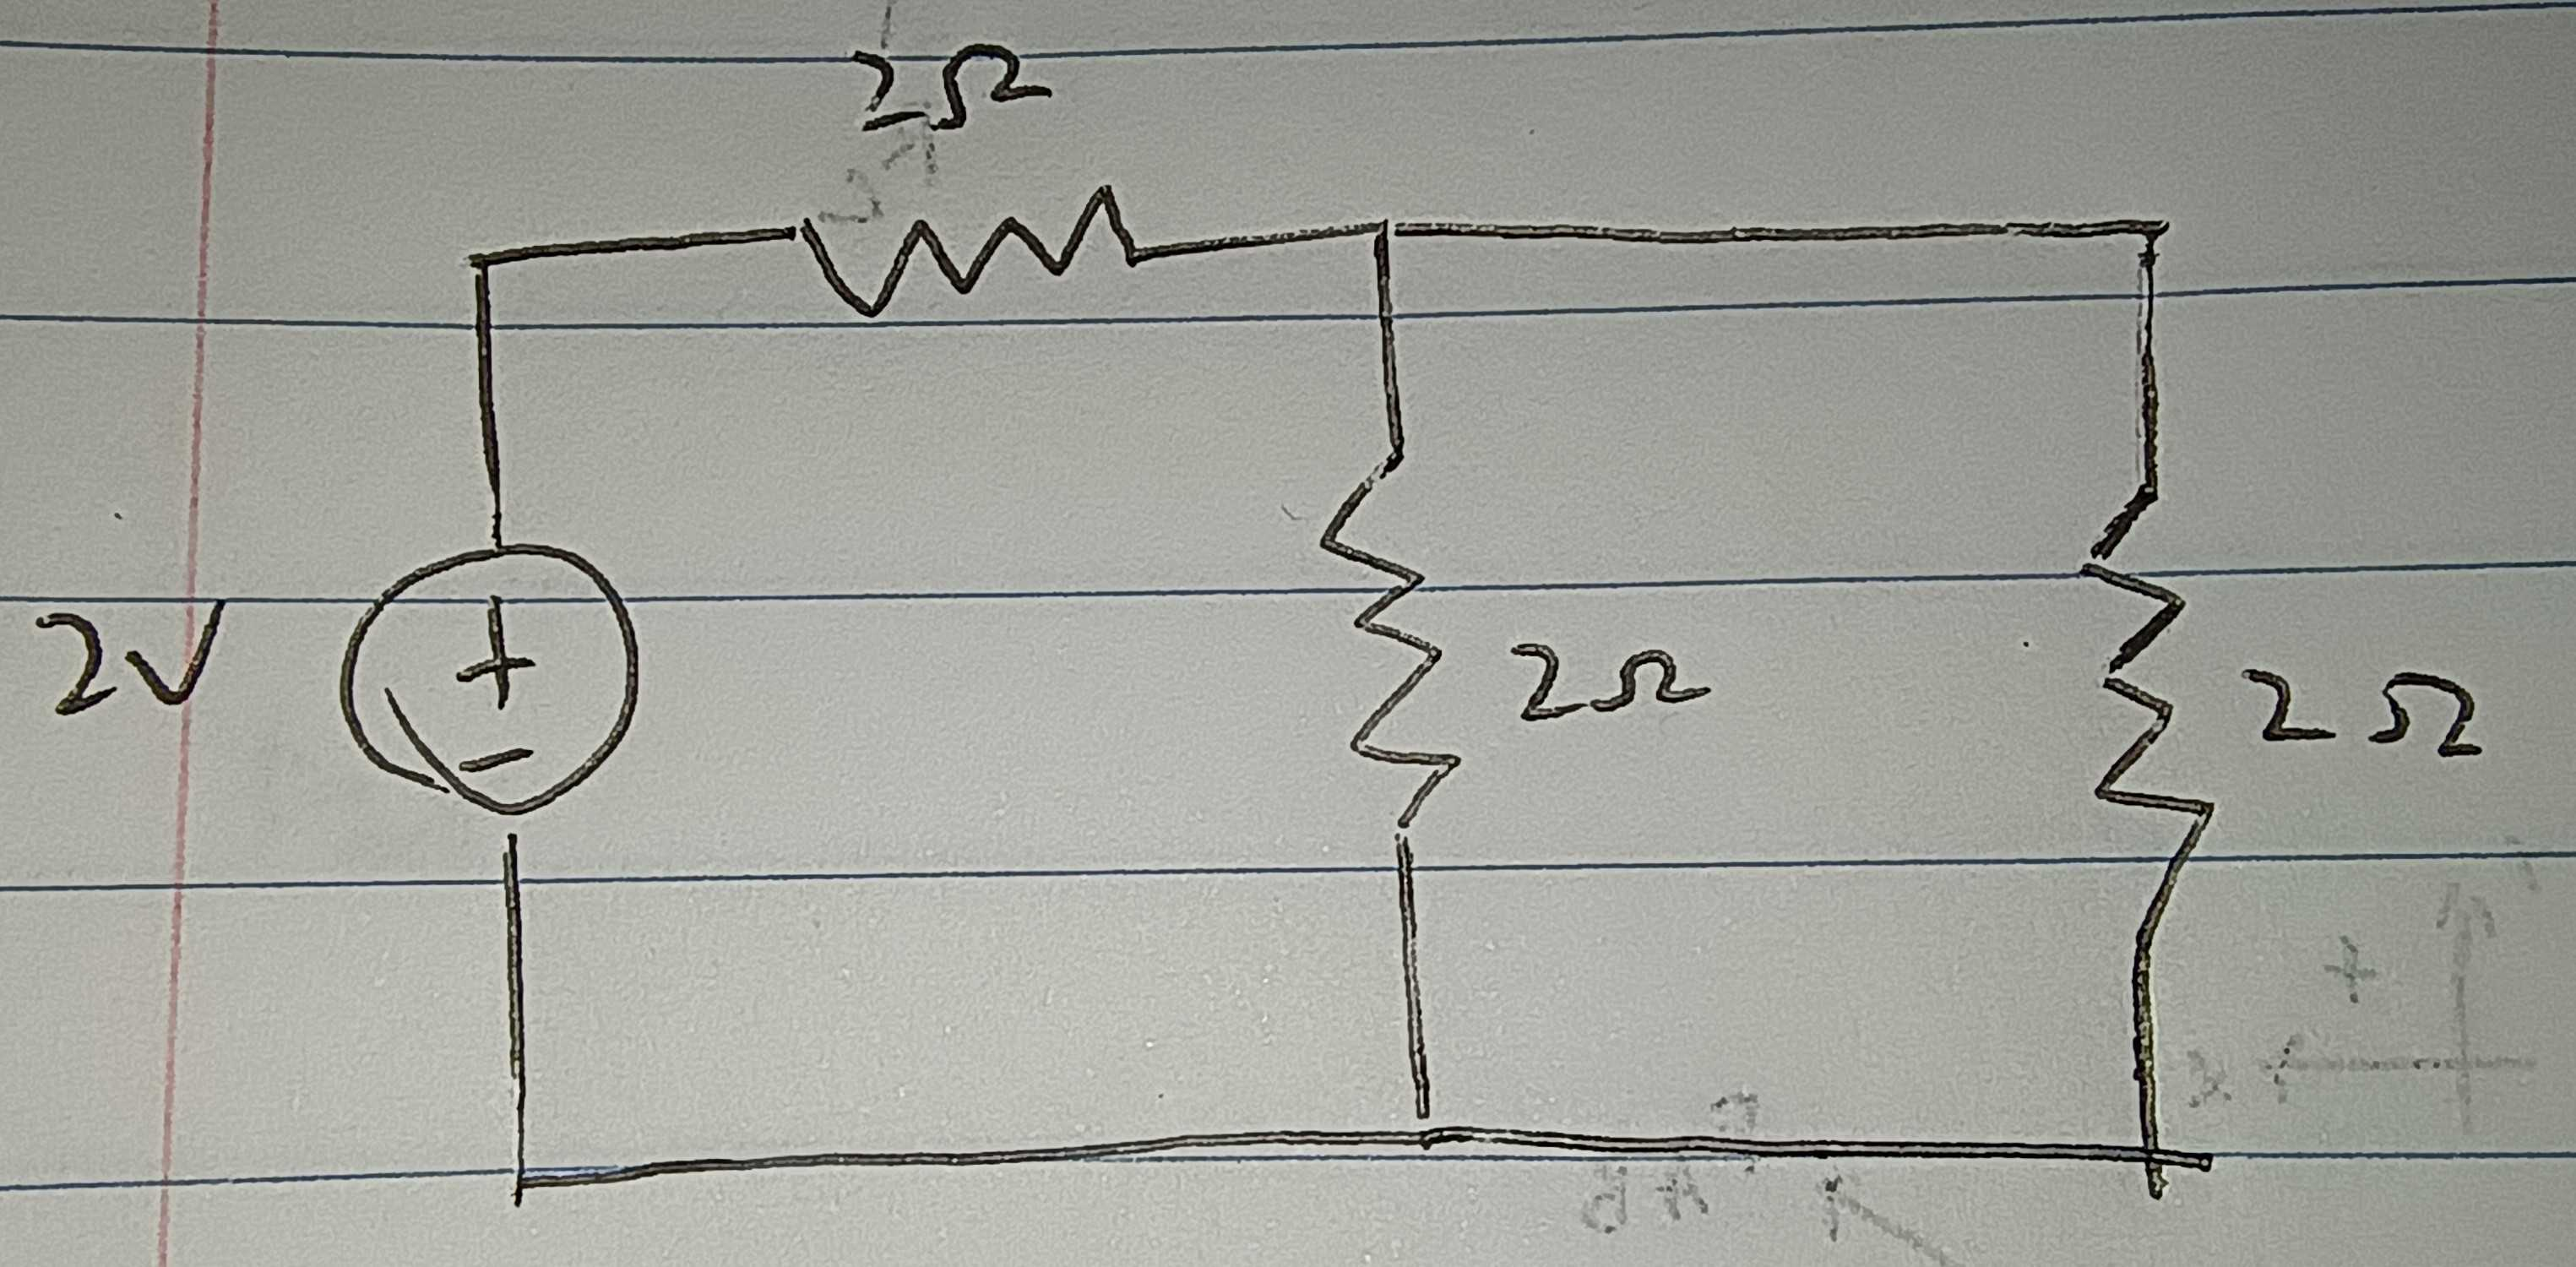
\includegraphics[width=0.6\textwidth]{5-5-2.jpg}
\end{center}
Combine the parallel resistors:
\[R_{\text{eq}} = \frac{[2+2\,\Omega]}{[2\cdot2\,\Omega]} = 1\,\Omega\]
Use voltage division to find voltage across the 1 $\Omega$ resistor:
\[v_1 = [2\,\text{V}]\frac{[1\,\Omega]}{[1+2\,\Omega]} = 0.6666\,\text{V}\]
This is the same voltage across the original 2 $\Omega$ resistor, so we can find the current through it:
\[i_x'' = \frac{v_1}{[2\,\Omega]} = \frac{0.6666}{2} = 0.3333\,\text{A}\]
Superposition:
\[\boxed{i_x = i_x' + i_x'' = [0.3333 + 0.3333\,\text{A}] = 0.6666\,\text{A}}\]
\textbf{(b)}\\
The current contributions are equal so its 50\% from the voltage source and 50\% from the current source.
\textbf{(c)} To double the current, the contribution from the current source will have to be $i_x' = 1\,\text{A}$.\\
\[\boxed{i_x' = [1\,\text{A}] =\frac{[1\,\Omega]}{[1+2\,\Omega]} \cdot i_s \quad\implies\quad i_s = 3\,\text{A}}\]

\section*{5.11}
\vspace{-2em}
\begin{center}
    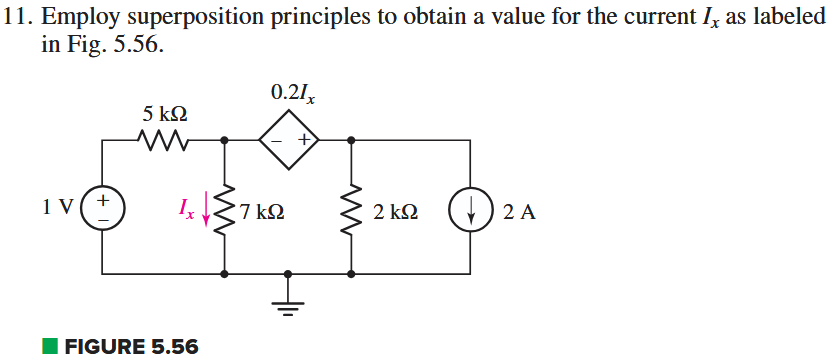
\includegraphics[width=0.8\textwidth]{5-11.png}
\end{center}
\vspace{-1em}
Isolating current source:
\begin{center}
    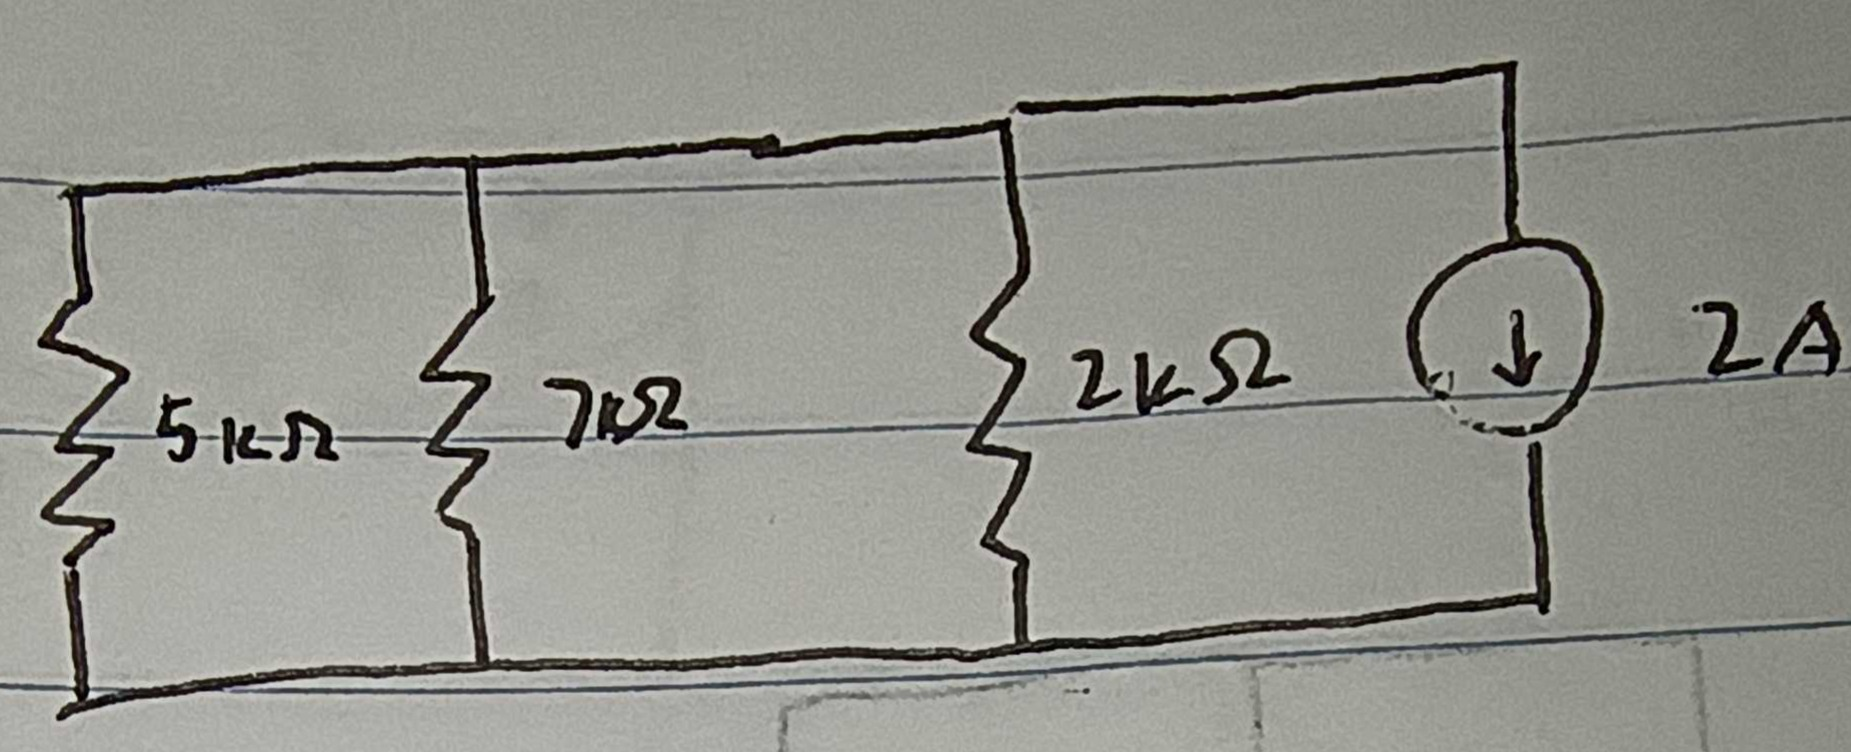
\includegraphics[width=0.6\textwidth]{5-11-1.jpg}
\end{center}
Combining the parallel resistors:
\[\frac{1}{R_{\text{eq}}} = \frac{1}{[2\,k\Omega]} + \frac{1}{[7\,k\Omega]} = \frac{1}{[5\,k\Omega]} \quad\implies\quad R_{\text{eq}} = 1.1864\,k\Omega\]
\[\implies v = [2\,\text{A}] \cdot [1.1864\,k\Omega] = 2.3728\,\text{V}\]
This is equal to the voltage over the 7 k$\Omega$ resistor, so we can find the current through it:
\[I_x' = \frac{v}{[7\,k\Omega]} = \frac{2.3728}{7000} = 3.389\times10^{-4}\,\text{A} \uparrow\]
Isolating dependent voltage source:
\begin{center}
    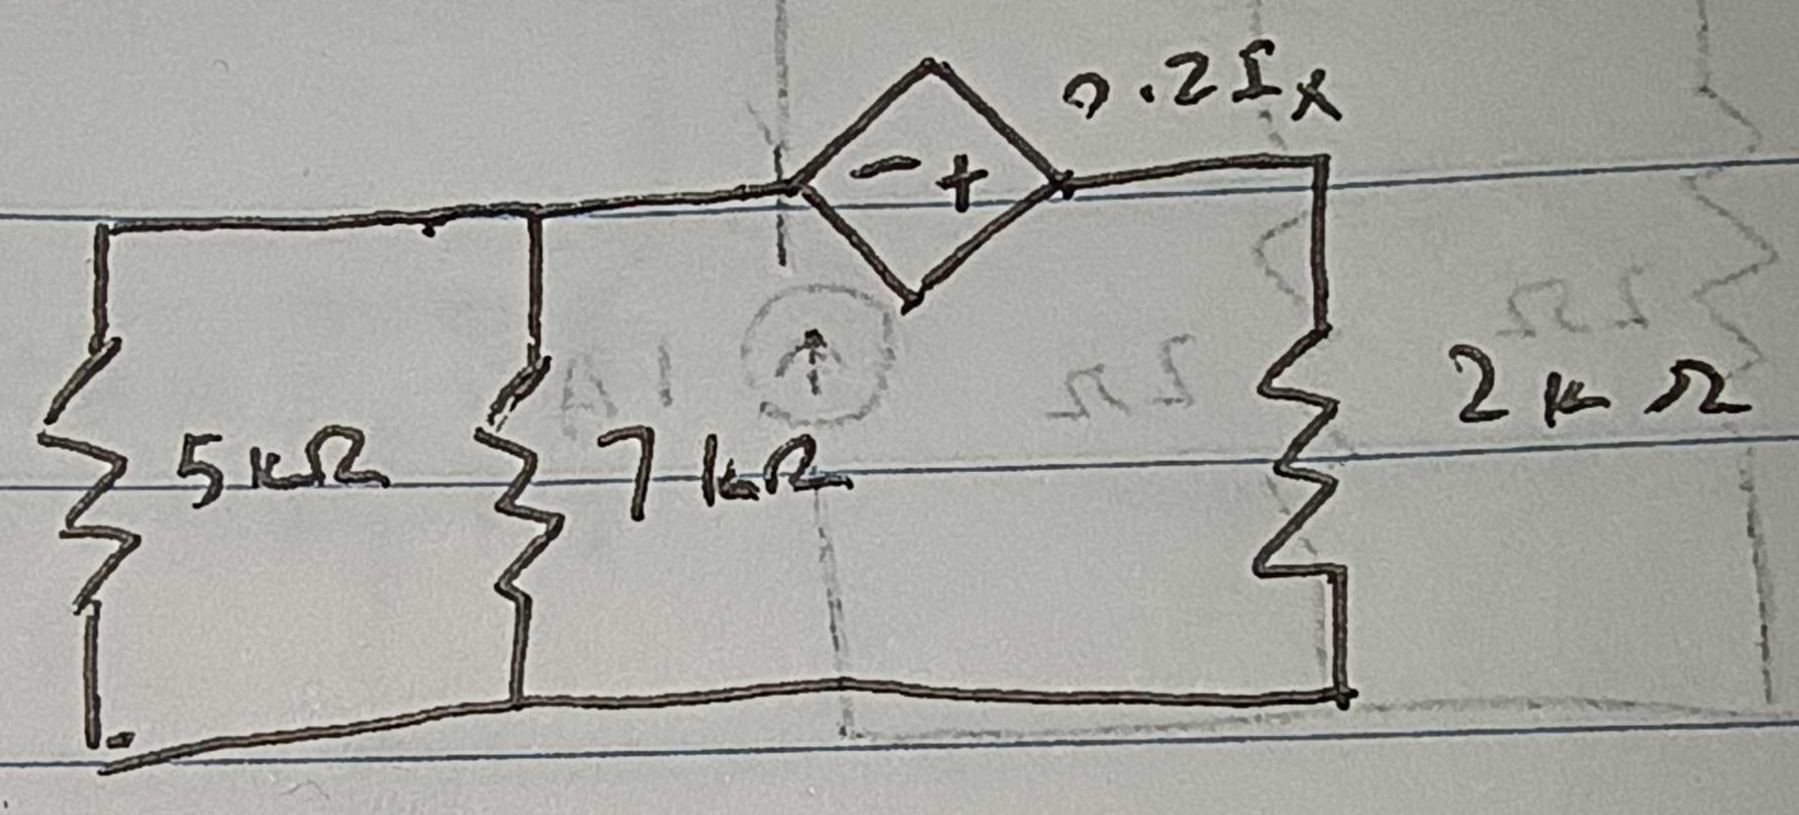
\includegraphics[width=0.6\textwidth]{5-11-2.jpg}
\end{center}
Combining the parallel resistors:
\[R_{\text{eq}} = \frac{[5\cdot7\,k\Omega]}{[5+7\,k\Omega]} = 2.9166\,k\Omega\]
Current voltage division:
\[v = \frac{[2916.6\,\Omega]}{[2916.6\,\Omega + 2000\,\Omega]} \cdot [0.2I_x\,\text{V}] = 0.1186I_x\,\text{V}\]
This is equal to the voltage across the 7 k$\Omega$ resistor, so we can find the current through it:
\[I_x'' = \frac{v}{[7\,k\Omega]} = \frac{0.1186I_x}{7000} = 1.6949\times10^{-5}I_x\,\text{A} \uparrow\]
Isolating independent voltage source:
\begin{center}
    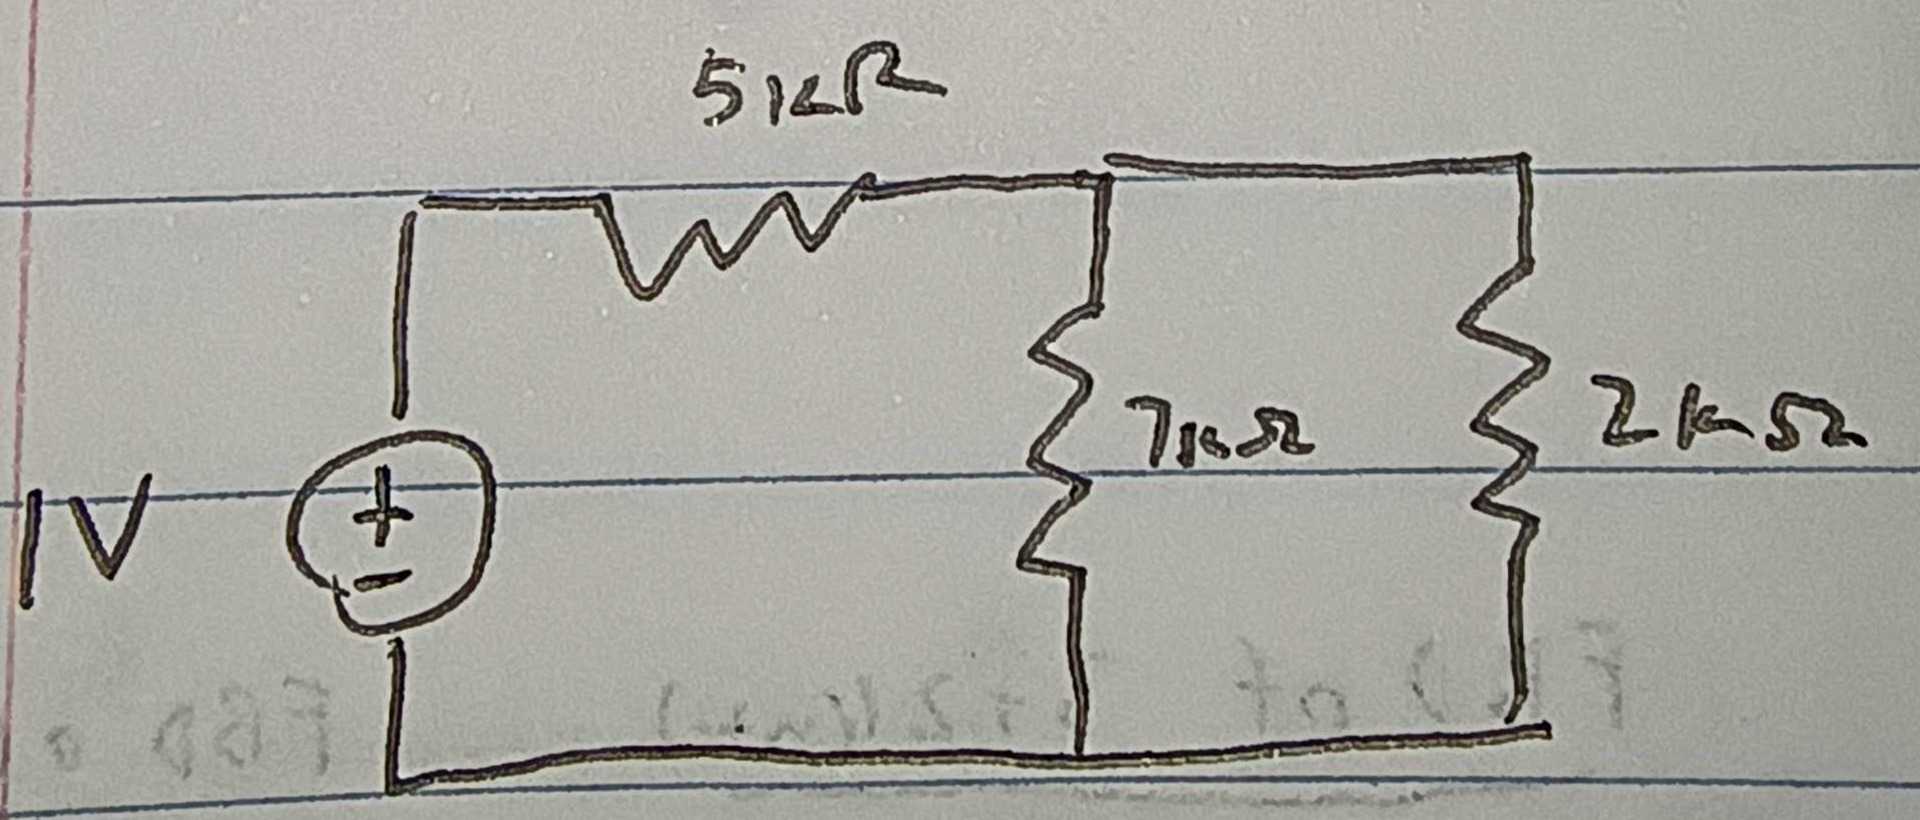
\includegraphics[width=0.6\textwidth]{5-11-3.jpg}
\end{center}
Combining the parallel resistors:
\[R_{\text{eq}} = \frac{[2\cdot7\,k\Omega]}{[2+7\,k\Omega]} = 1.5555\,k\Omega\]
Current voltage division:
\[v = \frac{[1555.55\,\Omega]}{[1555.55\,\Omega + 5000\,\Omega]} \cdot [1\,\text{V}] = 0.2372\,\text{V}\]
This is equal to the voltage across the 7 k$\Omega$ resistor, so we can find the current through it:
\[I_x''' = \frac{v}{[7\,k\Omega]} = \frac{0.2372}{7000} = 3.3898\times10^{-5}\,\text{A} \downarrow\]
Superposition:
\[I_x = I_x' + I_x'' + I_x''' = [3.389\times10^{-4} + 1.6949\times10^{-5}I_x - 3.3898\times10^{-5}\,\text{A}]\]
\[\implies 0.9999I_x = 3.2262\times10^{-4}\,\text{A}\quad\implies\quad \boxed{I_x = 3.0500\times10^{-4}\,\text{A} \uparrow}\]

\section*{5.18}
\vspace{-2em}
\begin{center}
    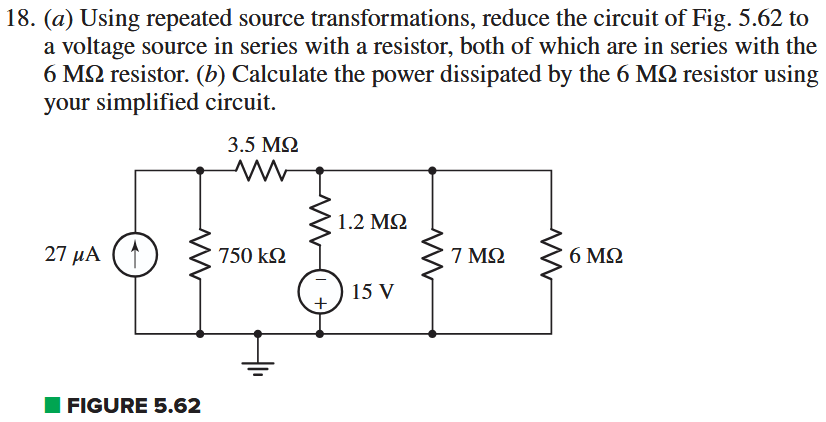
\includegraphics[width=0.8\textwidth]{5-18.png}
\end{center}
\vspace{-1em}
\textbf{(a)} Goal: put everything in parallel to each other with 2 current sources and 2 resistors (one of them being 6 M$\Omega$).\\
Starting by transforming the voltage source into a current source:
\begin{center}
    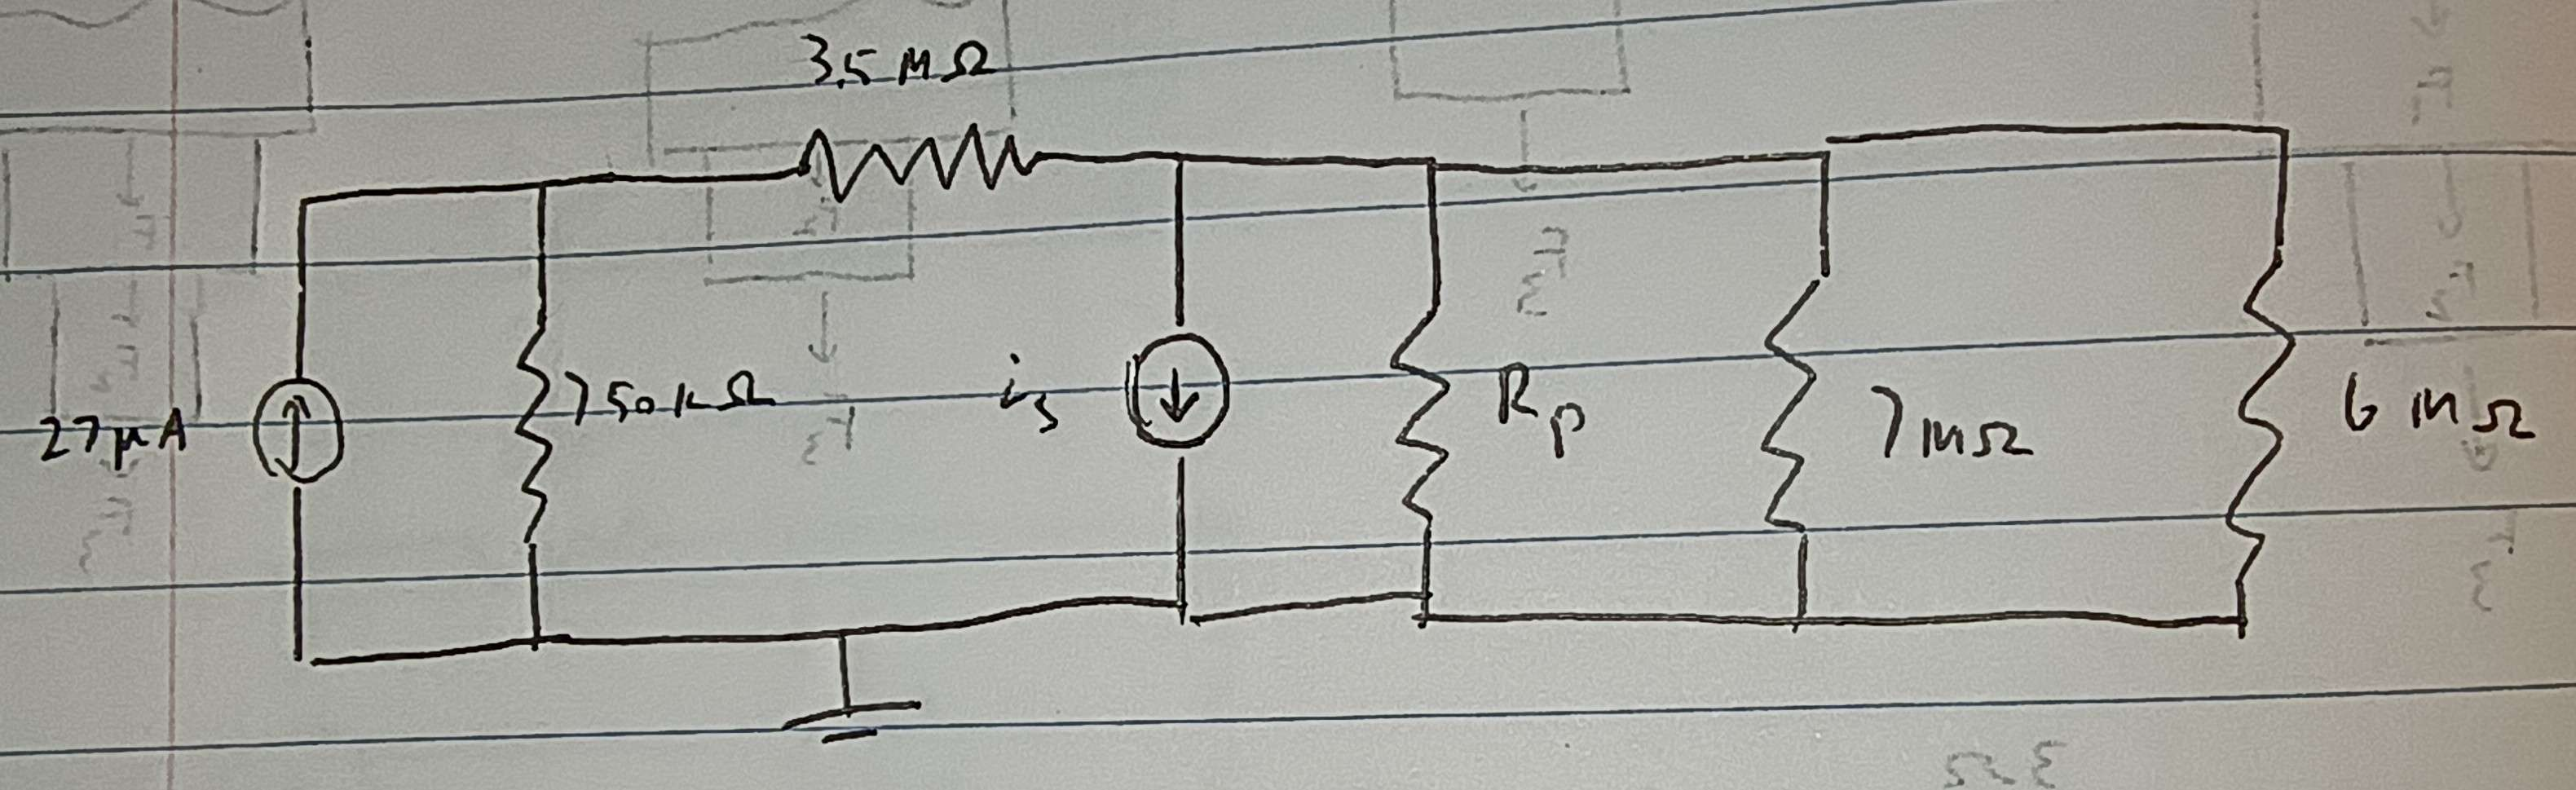
\includegraphics[width=0.8\textwidth]{5-18-1.jpg}
\end{center}
\[R_s = R_p \quad\implies\quad R_p  = 1.2\,M\Omega\]
\[v_s = i_s R_s \quad\implies\quad i_s = \frac{[15\,\text{V}]}{[1.2\,M\Omega]} = 12.5\times10^{-6}\,\text{A}\]
Converting the 27 $\mu$A current source to a voltage source:
\begin{center}
    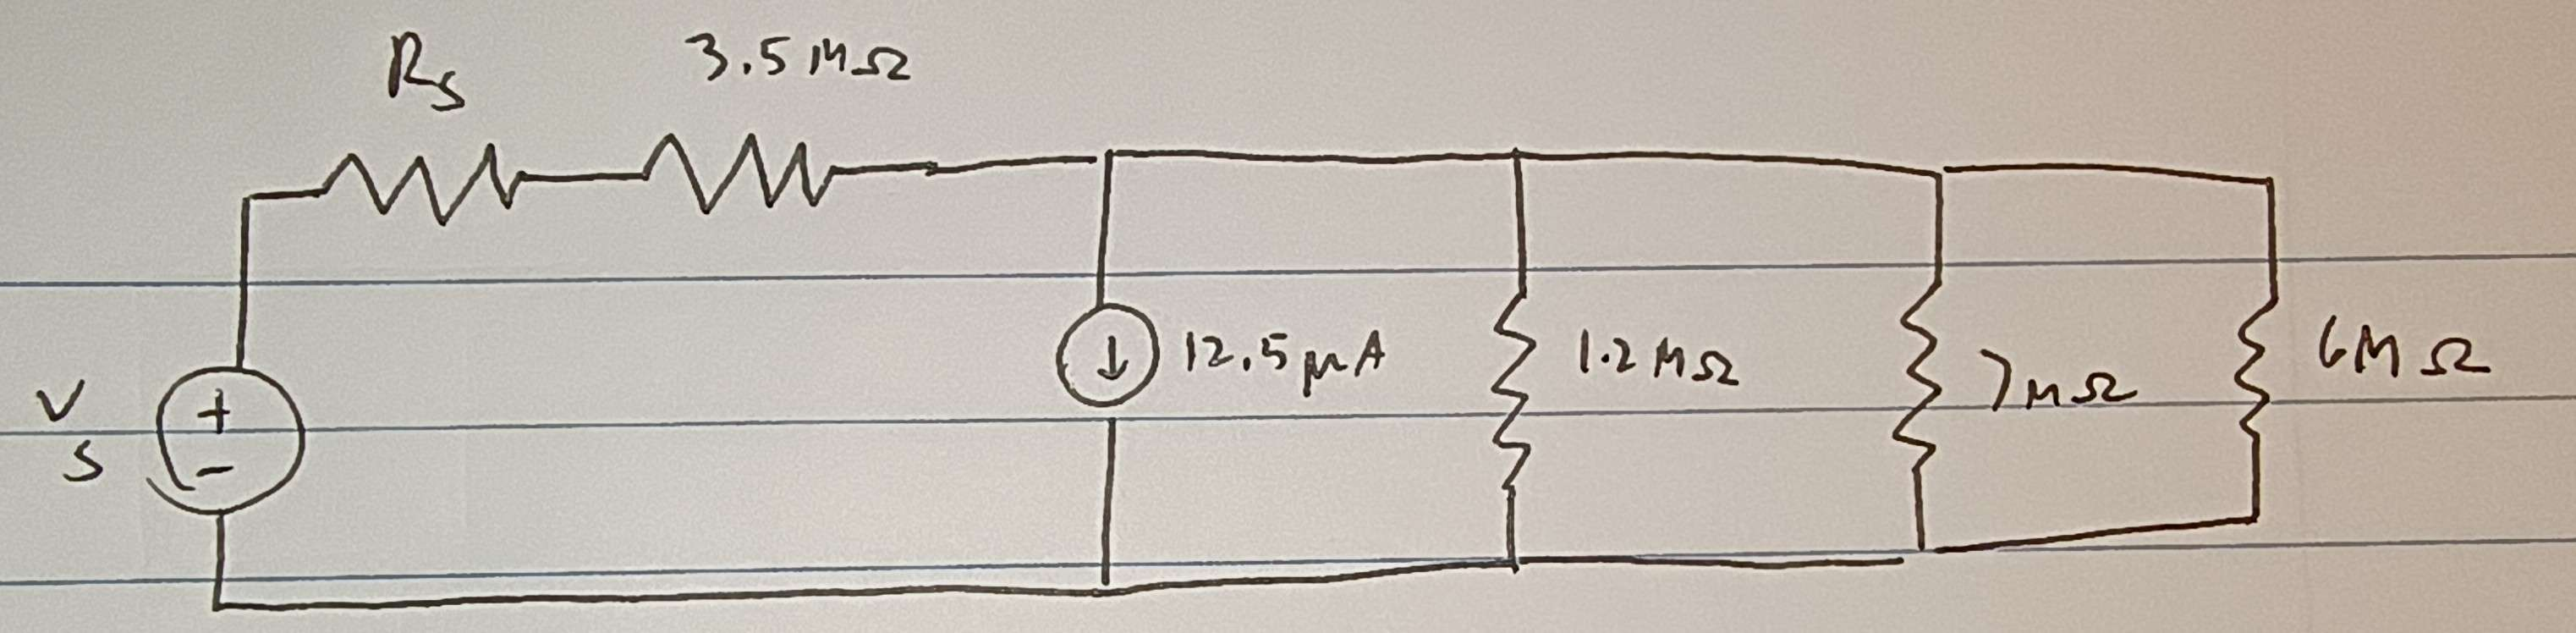
\includegraphics[width=0.8\textwidth]{5-18-2.jpg}
\end{center}
\[R_s = R_p \quad\implies\quad R_s = 750\,k\Omega\]
\[v_s = i_s R_s \quad\implies\quad v_s = [27\times10^{-6}\,\text{A}] \cdot [750\times10^3\,\Omega] = 20.25\,\text{V}\]
Now we can combine the two resistors in series:
\[R = [750\times10^3\,\Omega] + [3.5\times10^6\,\Omega] = 4.25\times10^6\,\Omega\]
A the 20.25 V voltage source is in series with the 4.25 M$\Omega$ resistor, we can convert it to a current source:
\[R_s = R_p \quad\implies\quad R_p = 4.25\,M\Omega\]
\[v_s = i_s R_s \quad\implies\quad i_s = \frac{[20.25\,\text{V}]}{[4.25\,M\Omega]} = 4.7647\times10^{-6}\,\text{A}\]
Now everything is in parallel:
\begin{center}
    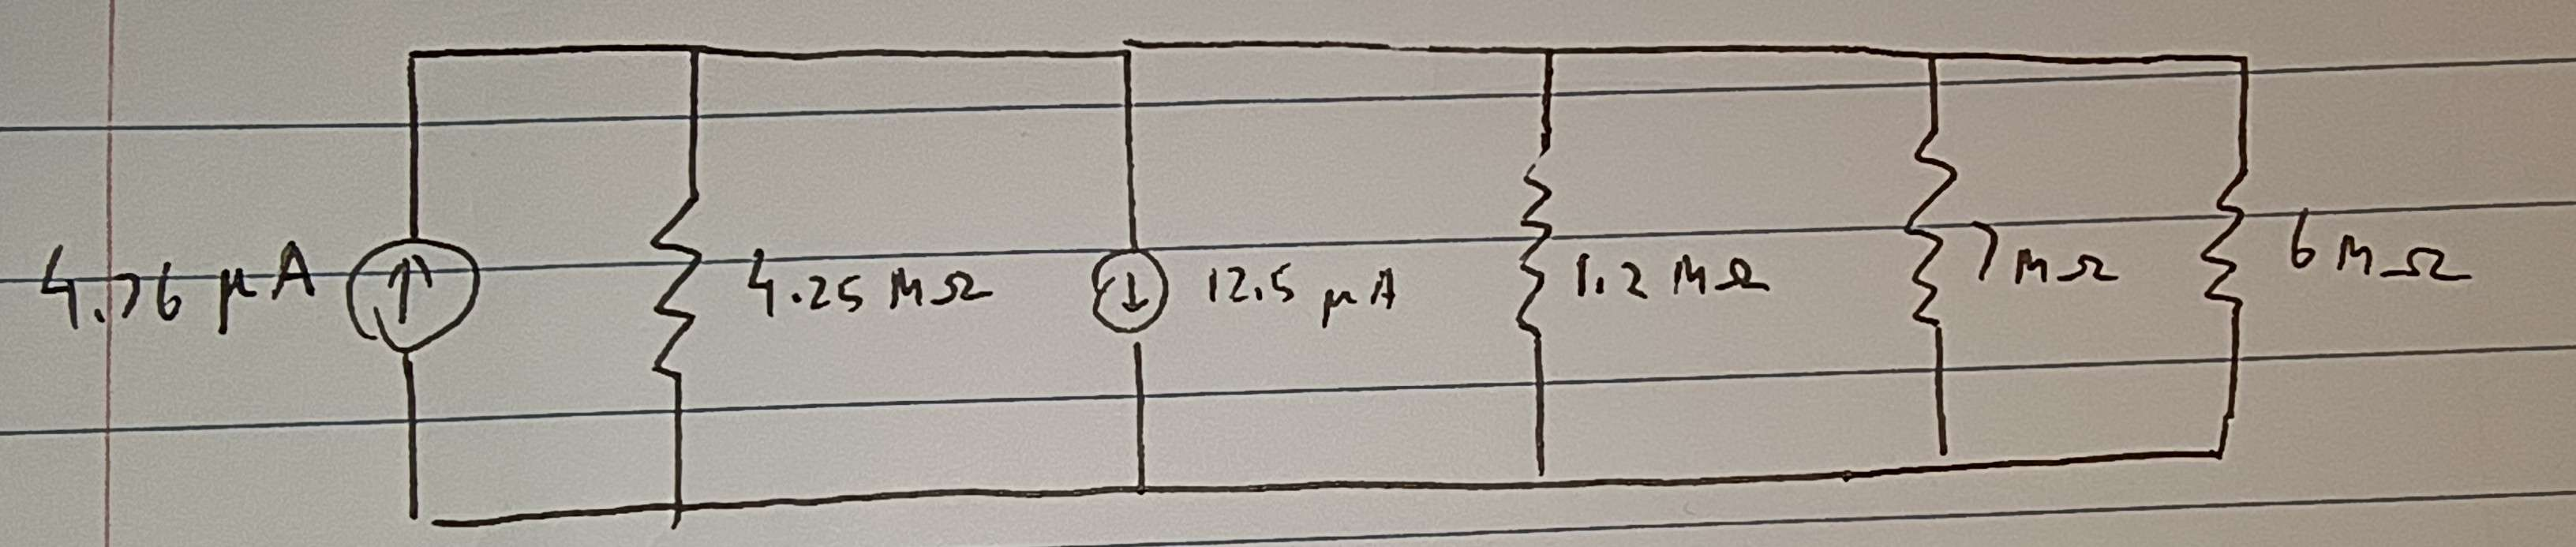
\includegraphics[width=0.8\textwidth]{5-18-3.jpg}
\end{center}
Combine the parallel current sources (taking up as positive):
\[i_{\text{eq}} = [4.7647\times10^{-6}\,\text{A}] - [12.5\times10^{-6}\,\text{A}] = -7.7353\times10^{-6}\,\text{A}\]
Combining the parallel resistors (except the 6 M$\Omega$ one):
\[\frac{1}{R_{\parallel}} = \frac{1}{[4.25\times10^6\,\Omega]} + \frac{1}{[1.2\times10^6\,\Omega]} + \frac{1}{[7\times10^6\,\Omega]}\quad\implies\quad R_{\parallel} = 8.2543\times10^5\,\Omega\]
This can finally be converted to a voltage source:
\[R_s = R_p \quad\implies\quad R_s = 8.2543\times10^5\,\Omega\]
\[v_s = i_s R_s \quad\implies\quad v_s = [-7.7353\times10^{-6}\,\text{A}] \cdot [8.2543\times10^5\,\Omega] = -6.3849\,\text{V}\]
\begin{center}
    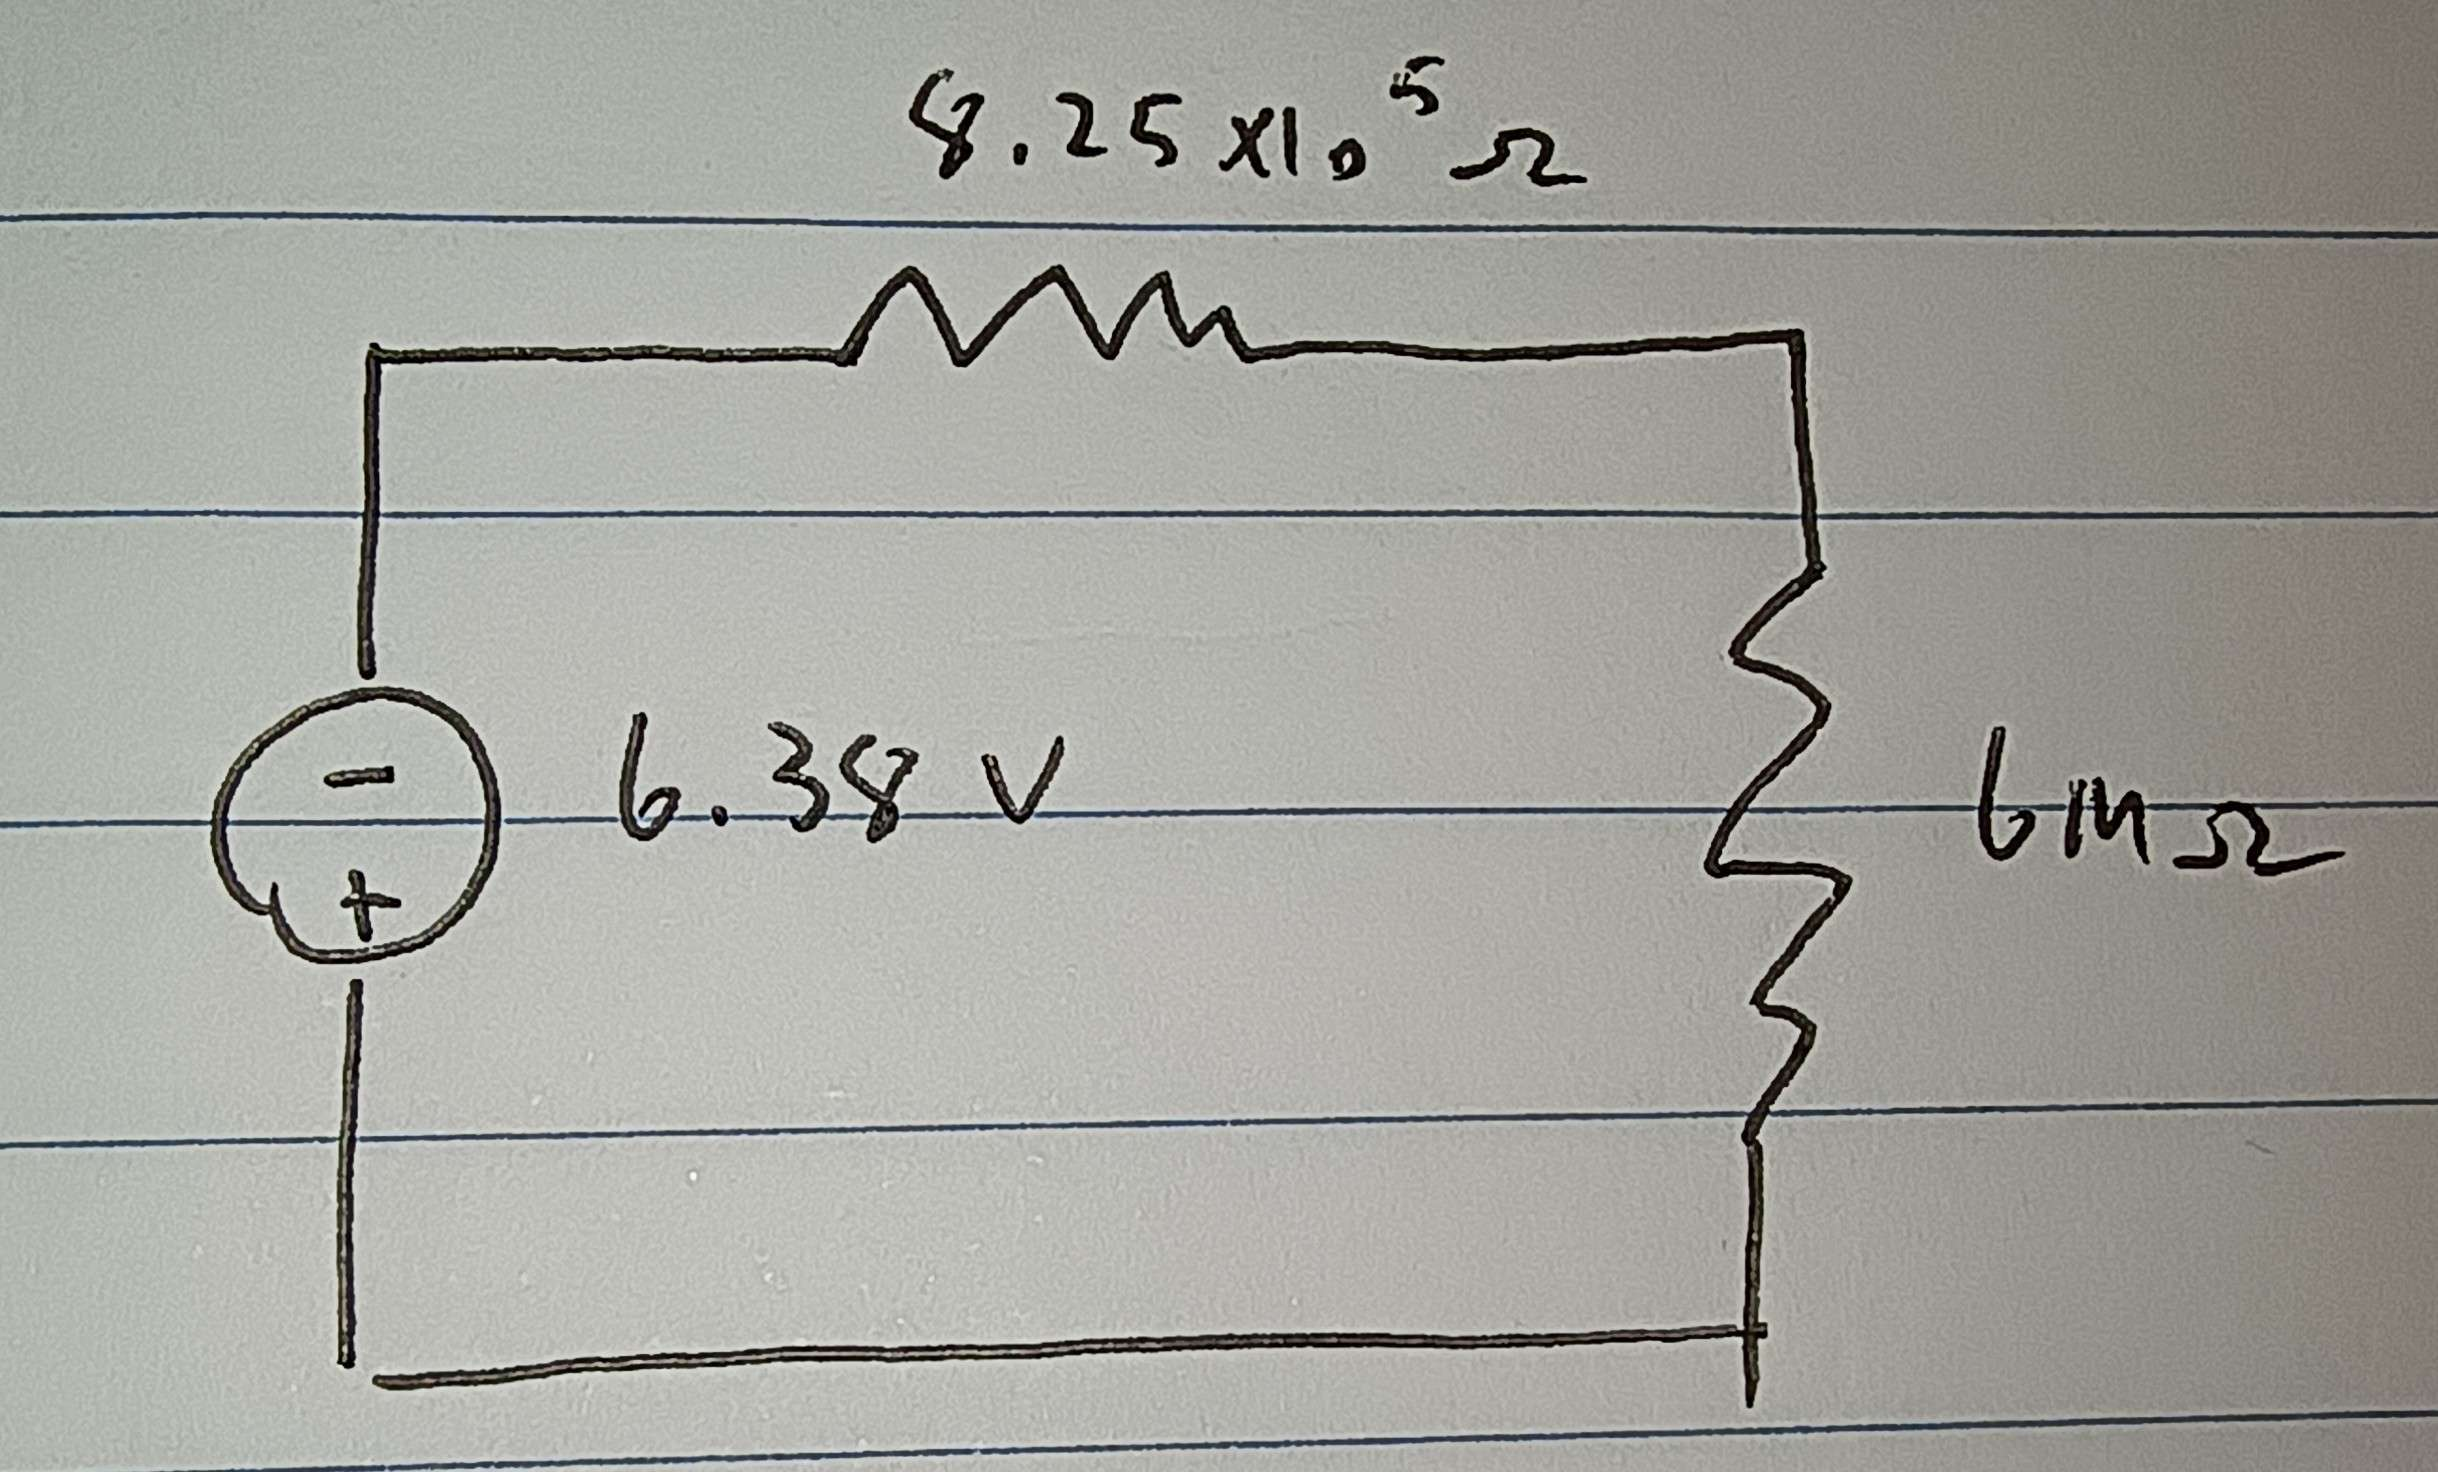
\includegraphics[width=0.5\textwidth]{5-18-4.jpg}
\end{center}
\textbf{(b)} Using voltage division to find voltage across the 6 M$\Omega$ resistor:
\[v = \frac{[6\times10^6\,\Omega]}{[6\times10^6\,\Omega + 8.2543\times10^5\,\Omega]} \cdot [6.3849\,\text{V}] = 5.6127\,\text{V}\]
Power dissipated by the 6 M$\Omega$ resistor:
\[P = \frac{v^2}{R} = \frac{[5.6127\,\text{V}]^2}{[6\times10^6\,\Omega]} = \boxed{5.25\times10^{-6}\,\text{W}}\]

\end{document}